\documentclass[final]{article}

\usepackage[paperwidth=594mm,paperheight=841mm,margin=14mm]{geometry}
\usepackage[T1]{fontenc}
\usepackage[utf8]{inputenc}
\usepackage[english]{babel}
\usepackage{lmodern}
\usepackage{amsmath,amssymb}
\usepackage{booktabs}
\usepackage{tikz}
\usepackage{pgfplots}
\usepackage{xcolor}
\usepackage{array}
\usepackage{graphicx}

\renewcommand{\familydefault}{\sfdefault}
\pgfplotsset{compat=1.18}
\pagestyle{empty}
\setlength{\parindent}{0pt}
\setlength{\parskip}{0.30em}

\definecolor{dmblue}{HTML}{3F7DF1}
\definecolor{softblue}{HTML}{EAF2FF}
\definecolor{softgreen}{HTML}{EAF8EF}
\definecolor{softred}{HTML}{FFF0EE}
\definecolor{goodgreen}{HTML}{209B3A}
\definecolor{warnred}{HTML}{D3342F}
\definecolor{textgray}{HTML}{50545C}
\definecolor{linegray}{HTML}{AEB4BE}
\definecolor{lightgray}{HTML}{F5F7FA}

% -----------------------------
% Editable experiment numbers.
% CrossPlay values are measured from the current checkpoint evaluation.
% Self-play values are placeholders following the stated assumption that
% both self-play baselines are slightly weaker than CrossPlay.
% -----------------------------
\newcommand{\initAWin}{0.008}
\newcommand{\initBWin}{0.084}
\newcommand{\initTie}{0.908}
\newcommand{\crossAWin}{0.340}
\newcommand{\crossBWin}{0.516}
\newcommand{\crossTie}{0.144}
\newcommand{\crossAReward}{0.1429}
\newcommand{\crossBReward}{0.1721}
\newcommand{\selfQwenReward}{0.083}
\newcommand{\selfSmolReward}{0.132}
\newcommand{\selfQwenWin}{0.285}
\newcommand{\selfSmolWin}{0.465}

\newcommand{\BlockTitle}[1]{%
  {\color{dmblue}\fontsize{32}{36}\selectfont\bfseries #1}\par
  \vspace{0.08em}{\color{linegray}\rule{\linewidth}{1.2pt}}\vspace{0.24em}
}

\newcommand{\MiniTitle}[1]{%
  {\color{dmblue}\fontsize{25}{29}\selectfont\bfseries #1}\par
  \vspace{0.15em}
}

\newcommand{\Key}[1]{{\bfseries #1}}
\newcommand{\Good}[1]{{\color{goodgreen}#1}}
\newcommand{\Bad}[1]{{\color{warnred}#1}}

\newcommand{\PosterBlock}[2]{%
  \begin{minipage}[t]{\linewidth}
  \BlockTitle{#1}
  {\fontsize{20.5}{25}\selectfont #2}
  \end{minipage}
}

\newcommand{\SmallNote}[1]{{\fontsize{16}{19}\selectfont\color{textgray}#1}}
\newcommand{\ResultPlotHeight}{130mm}
\newcommand{\ResultPlotWidth}{0.86\linewidth}
\newcommand{\ResultTable}[1]{%
  \begin{center}
  {\color{black}\fontsize{22.5}{26}\selectfont
   \setlength{\tabcolsep}{2.4pt}
   \renewcommand{\arraystretch}{1.24}#1}
  \end{center}
}

\begin{document}

\begin{center}
  {\fontsize{31}{35}\selectfont\color{textgray}\bfseries Heterogeneous Preference Training}\par
  \vspace{0.18em}
  {\fontsize{48}{54}\selectfont\color{dmblue}\bfseries Dynamic Opponents Improve Preference Training in Heterogeneous LLM Cross-Play}\par
  \vspace{0.25em}
  {\fontsize{23}{27}\selectfont
  Vasyagina Ekaterina, MIPT \quad $\cdot$ \quad Qwen2.5-0.5B-Instruct vs. SmolLM2-1.7B-Instruct on GSM8K}
\end{center}

\vspace{0.30em}

\begin{minipage}[t]{0.487\linewidth}
\PosterBlock{TL;DR}{
\Key{What?} We study heterogeneous online preference training: Qwen and SmolLM answer the same GSM8K prompt, a verifier converts their answers into a preference pair, and both policies are updated with DPO.

\Key{Why?} In self-play, comparisons are drawn from one model family or a fixed reference. A \Good{live heterogeneous opponent} changes the preference-pair distribution and exposes different reasoning and formatting errors.

\Key{How?} The comparison is controlled by matching exposure for both policies:
\[
\Delta_{\mathrm{replay}}=\Delta_{\mathrm{pairs}}=\Delta_{\mathrm{updates}}=0.
\]

\Key{Result.} At checkpoint 1000, CrossPlay reaches validation win rates $0.340/0.516$ for Qwen/SmolLM and higher verifier rewards than the corresponding self-play baselines.
}

\vspace{0.42em}

\PosterBlock{Background: From RLHF to Games}{
Preference optimization usually starts from pairs $(y^+,y^-)$ and updates a policy relative to a reference. DPO makes this practical by replacing PPO-style reward optimization with a contrastive objective.

NLHF reframes alignment as a game over pairwise preferences:
\[
p_\phi(x,y,y')=P(y\succ y'\mid x),
\]
and seeks a policy that is robust against competing policies. Online IPO and SPPO show that online preference sampling and self-play can be connected to Nash-style equilibria.

\Key{Question.} Does changing the live opponent model improve the preference data used for training, when data volume and update counts are held fixed?
}

\vspace{0.42em}

\PosterBlock{Why Dynamic Opponents?}{
\begin{center}
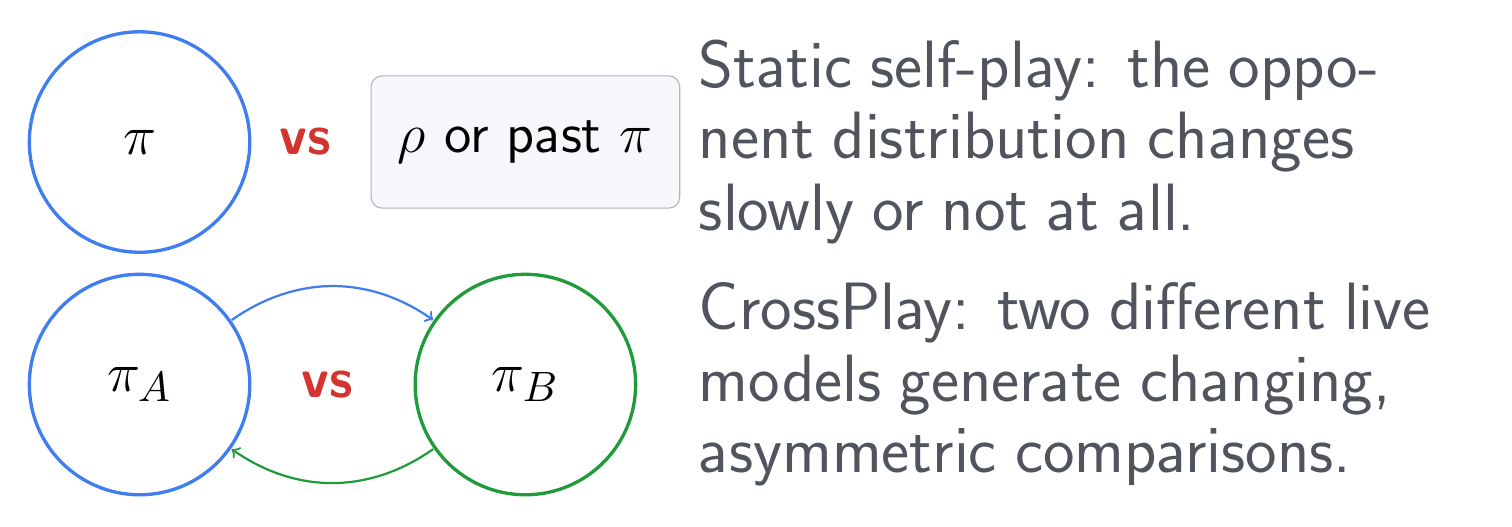
\begin{tikzpicture}[font=\fontsize{15.5}{18.5}\selectfont,scale=1.40,transform shape]
  \node[draw=dmblue,circle,very thick,minimum size=20mm] (p) at (-3.7,0) {$\pi$};
  \node[draw=linegray,rounded corners=4pt,fill=lightgray,minimum width=28mm,minimum height=12mm] (ref) at (-0.2,0) {$\rho$ or past $\pi$};
  \node at (-2.2,0) {\color{warnred}\bfseries vs};
  \node[anchor=west,text width=70mm] at (1.25,0) {\SmallNote{Static self-play: the opponent distribution changes slowly or not at all.}};

  \node[draw=dmblue,circle,very thick,minimum size=20mm] (pa) at (-3.7,-2.2) {$\pi_A$};
  \node[draw=goodgreen,circle,very thick,minimum size=20mm] (pb) at (-0.2,-2.2) {$\pi_B$};
  \node at (-2.0,-2.2) {\color{warnred}\bfseries vs};
  \draw[->,thick,dmblue,bend left=35] (pa) to (pb);
  \draw[->,thick,goodgreen,bend left=35] (pb) to (pa);
  \node[anchor=west,text width=70mm] at (1.25,-2.2) {\SmallNote{CrossPlay: two different live models generate changing, asymmetric comparisons.}};
\end{tikzpicture}
\end{center}

\Key{Hypothesis.} A heterogeneous opponent changes the online preference distribution $q_t(y^+,y^-\mid x)$, producing comparisons that are less tied to one model's own error profile.

\Key{Control.} Replay entries, selected pairs, and optimizer steps are equalized; the intended experimental variable is the opponent distribution.
}

\vspace{0.42em}

\PosterBlock{Verifier-based Preference Construction}{
For each prompt $x$, both models generate answers $y_A,y_B$. 
A dense GSM8K verifier extracts the final answer $\hat a_i$ and assigns a score $s_i$.

{\fontsize{19.2}{22.2}\selectfont
\[
\begin{gathered}
r_i^{\mathrm{bad}}
=
\min\!\left(
0.30,\,
\max(0.02m_i,0.05h_i)+0.03h_i+0.20h_iq_i
\right),
\\[-1mm]
s_i
=
\mathbf{1}\{\hat a_i=a^\star\}
+
\mathbf{1}\{\hat a_i\ne a^\star\}r_i^{\mathrm{bad}},
\\[-1mm]
q_i
=
\left(
1+\frac{|\hat a_i-a^\star|}{\max(|a^\star|,1)}
\right)^{-1},
\qquad
q_i=0\ \mathrm{if\ nonnumeric},
\\[-1mm]
m_i=\mathbf{1}\{\texttt{\#\#\#\#}\ \mathrm{parsed}\},
\qquad
h_i=\mathbf{1}\{\hat a_i\ \mathrm{extracted}\},
\\[-1mm]
y^+
=
\arg\max_{y_i\in\{y_A,y_B\}} s_i,
\qquad
y^-=\{y_A,y_B\}\setminus y^+ .
\end{gathered}
\]
}

The higher-scoring answer becomes the preferred response, producing the DPO pair $(y^+,y^-)$.
}

\end{minipage}
\hfill
\begin{minipage}[t]{0.487\linewidth}
\PosterBlock{Heterogeneous CrossPlay}{
\begin{center}
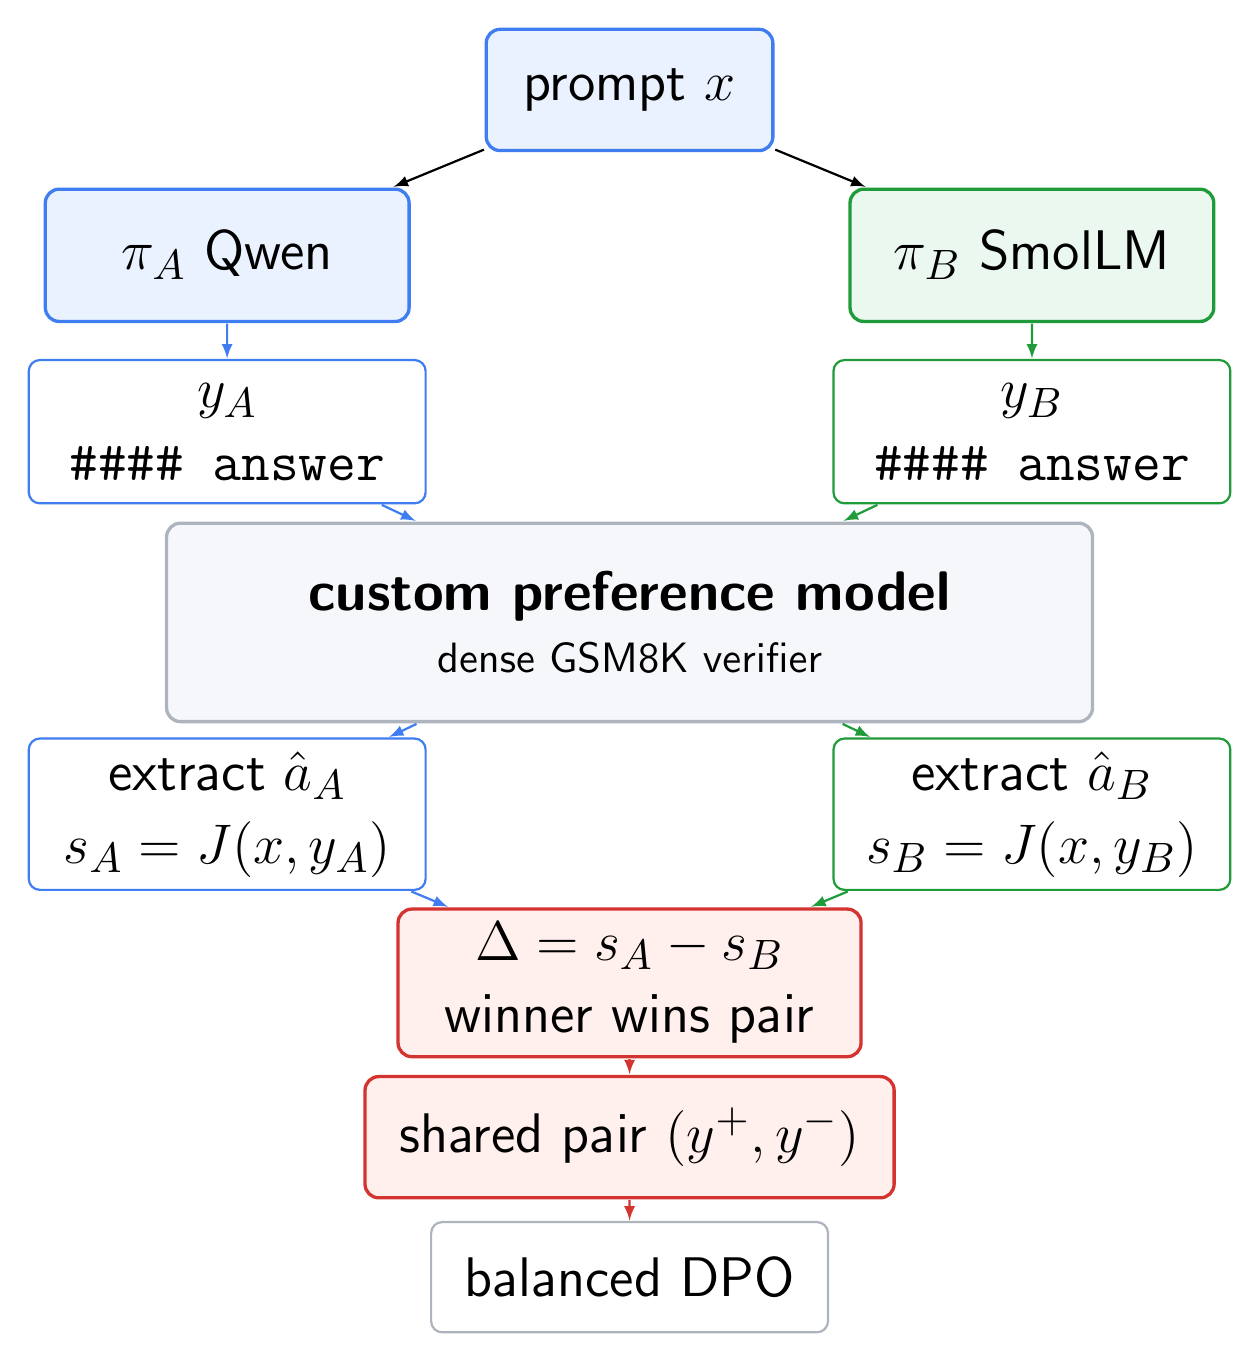
\begin{tikzpicture}[font=\fontsize{15.6}{18.8}\selectfont,>=latex,xscale=1.4,yscale=1.4,transform shape]
  \node[draw=dmblue,very thick,rounded corners=5pt,fill=softblue,minimum width=26mm,minimum height=11mm,align=center] (prompt) at (0,5.65) {prompt $x$};
  \node[draw=dmblue,very thick,rounded corners=5pt,fill=softblue,minimum width=33mm,minimum height=12mm,align=center] (a) at (-3.65,4.15) {$\pi_A$ Qwen};
  \node[draw=goodgreen,very thick,rounded corners=5pt,fill=softgreen,minimum width=33mm,minimum height=12mm,align=center] (b) at (3.65,4.15) {$\pi_B$ SmolLM};
  \node[draw=dmblue,thick,rounded corners=4pt,fill=white,minimum width=36mm,minimum height=13mm,align=center] (ya) at (-3.65,2.55) {$y_A$\\ \texttt{\#\#\#\# answer}};
  \node[draw=goodgreen,thick,rounded corners=4pt,fill=white,minimum width=36mm,minimum height=13mm,align=center] (yb) at (3.65,2.55) {$y_B$\\ \texttt{\#\#\#\# answer}};
  \node[draw=linegray,very thick,rounded corners=5pt,fill=lightgray,minimum width=84mm,minimum height=18mm,align=center] (pm) at (0,0.82) {\bfseries custom preference model\\[-1mm]{\fontsize{11}{13}\selectfont dense GSM8K verifier}};
  \node[draw=dmblue,thick,rounded corners=4pt,fill=white,minimum width=36mm,minimum height=12mm,align=center] (sa) at (-3.65,-0.92) {extract $\hat a_A$\\$s_A=J(x,y_A)$};
  \node[draw=goodgreen,thick,rounded corners=4pt,fill=white,minimum width=36mm,minimum height=12mm,align=center] (sb) at (3.65,-0.92) {extract $\hat a_B$\\$s_B=J(x,y_B)$};
  \node[draw=warnred,very thick,rounded corners=5pt,fill=softred,minimum width=42mm,minimum height=12mm,align=center] (cmp) at (0,-2.45) {$\Delta=s_A-s_B$\\winner wins pair};
  \node[draw=warnred,very thick,rounded corners=5pt,fill=softred,minimum width=48mm,minimum height=11mm,align=center] (pair) at (0,-3.85) {shared pair $(y^+,y^-)$};
  \node[draw=linegray,thick,rounded corners=4pt,fill=white,minimum width=36mm,minimum height=10mm,align=center] (upd) at (0,-5.12) {balanced DPO};

  \draw[->,thick] (prompt) -- (a);
  \draw[->,thick] (prompt) -- (b);
  \draw[->,thick,dmblue] (a) -- (ya);
  \draw[->,thick,goodgreen] (b) -- (yb);
  \draw[->,thick,dmblue] (ya) -- (pm);
  \draw[->,thick,goodgreen] (yb) -- (pm);
  \draw[->,thick,dmblue] (pm) -- (sa);
  \draw[->,thick,goodgreen] (pm) -- (sb);
  \draw[->,thick,dmblue] (sa) -- (cmp);
  \draw[->,thick,goodgreen] (sb) -- (cmp);
  \draw[->,thick,warnred] (cmp) -- (pair);
  \draw[->,thick,warnred] (pair) -- (upd);
\end{tikzpicture}
\end{center}

At training step $t$, a prompt $x_t\sim\mathcal{D}$ is answered by both live
policies, $y_i\sim\pi_i^t(\cdot\mid x_t)$ for $i\in\{A,B\}$. The verifier
constructs $(y^+,y^-)=C(x_t,y_A,y_B)$, and the same preference pair is used to
update each policy against its own frozen anchor $\rho_i$:
\[
z_i=\beta\!\left[
\log\frac{\pi_i(y^+\mid x_t)}{\pi_i(y^-\mid x_t)}
-\log\frac{\rho_i(y^+\mid x_t)}{\rho_i(y^-\mid x_t)}
\right],
\quad
\mathcal{L}_{i}=-\log\sigma(z_i).
\]
Replay entries, DPO pairs, and optimizer steps are matched across $A$ and $B$.
}

\vspace{2.42em}

\PosterBlock{Experimental Setup}{
{\fontsize{22.5}{26}\selectfont
\setlength{\tabcolsep}{3.2pt}
\renewcommand{\arraystretch}{1.14}
\begin{tabular}{@{}>{\bfseries}p{0.34\linewidth}p{0.60\linewidth}@{}}
Models & Qwen2.5-0.5B-Instruct, SmolLM2-1.7B-Instruct \\
Task & GSM8K math reasoning \\
Training subset & 2000 examples \\
Update & sigmoid DPO, $\beta=0.1$ \\
Batching & train batch $=1$, micro batch $=1$ \\
Responses & 128 tokens, final answer as \texttt{\#\#\#\# <answer>} \\
Reward & $1.0$ exact; otherwise dense score with format, answer, and numeric-proximity terms, capped at $0.30$ \\
Checkpoints & every 200 update steps \\
\end{tabular}
}
}

\vspace{0.42em}

\PosterBlock{Controlled Findings}{
\Key{1. Accounting control.} Replay entries, selected DPO pairs, and update steps are equalized for both policies.

\Key{2. Training signal.} CrossPlay improves validation win rate and dense verifier reward over initialization; it also exceeds the provisional self-play baselines.

\Key{3. Scope.} The current system uses a dense GSM8K verifier rather than a learned human-preference model, so it is an NLHF-motivated approximation rather than full NLHF.
}
\end{minipage}

\vspace{5.2em}

{\color{linegray}\rule{\linewidth}{1.1pt}}
\vspace{0.35em}

{\color{dmblue}\fontsize{33}{38}\selectfont\bfseries Experimental Results}\par
\vspace{0.35em}

\begin{minipage}[t]{0.318\linewidth}
\MiniTitle{Initialization vs. CrossPlay}
\begin{center}
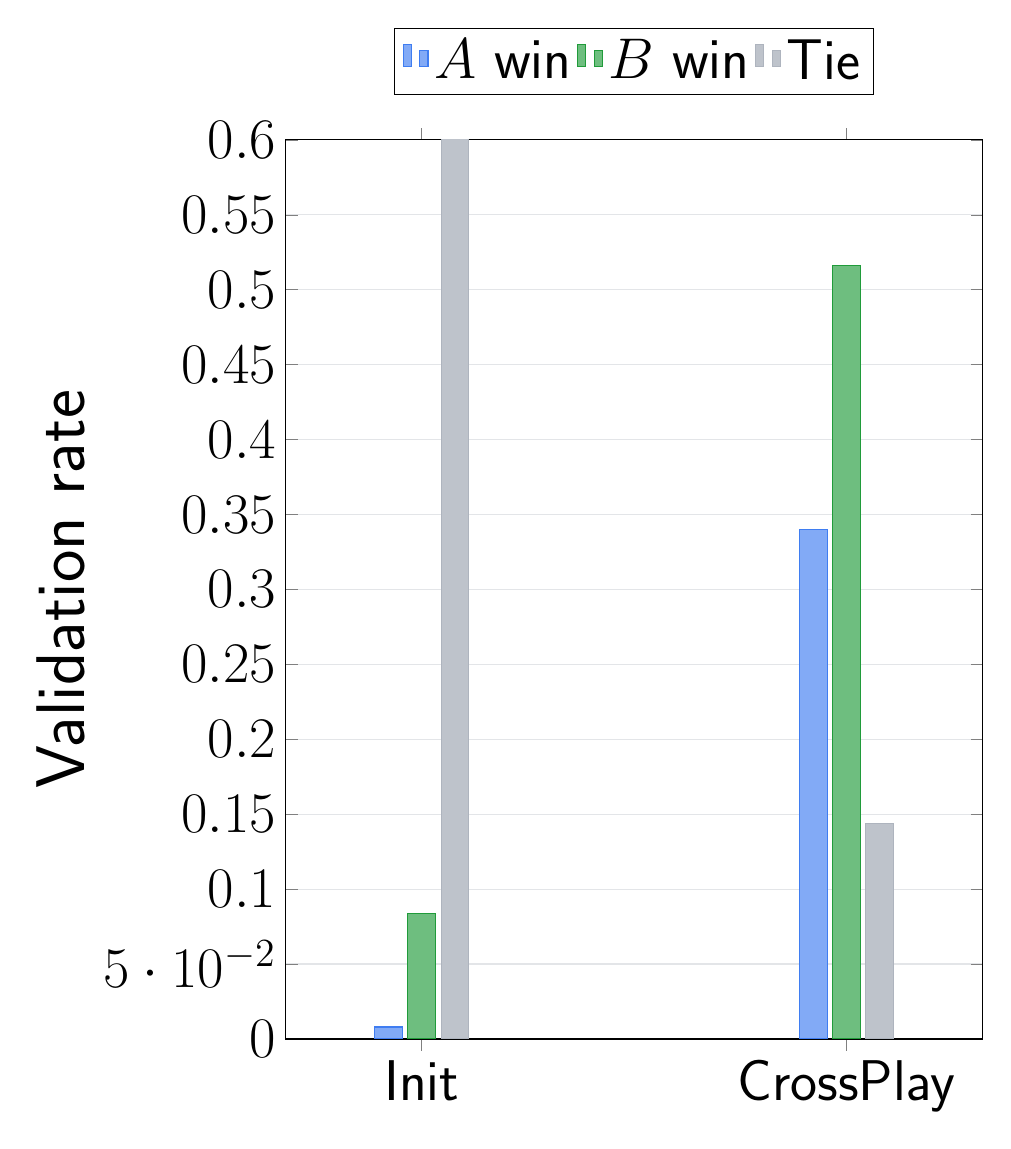
\begin{tikzpicture}
\begin{axis}[
  width=\ResultPlotWidth,
  height=\ResultPlotHeight,
  ybar,
  bar width=10pt,
  ymin=0,
  ymax=0.60,
  symbolic x coords={Init,CrossPlay},
  xtick=data,
  ylabel={Validation rate},
  ylabel style={font=\fontsize{23}{27}\selectfont},
  tick label style={font=\fontsize{21}{25}\selectfont},
  legend style={font=\fontsize{20}{24}\selectfont,at={(0.5,1.05)},anchor=south,legend columns=3},
  enlarge x limits=0.32,
  ymajorgrids=true,
  grid style={linegray!35}
]
\addplot+[fill=dmblue!65,draw=dmblue] coordinates {(Init,\initAWin) (CrossPlay,\crossAWin)};
\addplot+[fill=goodgreen!65,draw=goodgreen] coordinates {(Init,\initBWin) (CrossPlay,\crossBWin)};
\addplot+[fill=linegray!80,draw=linegray] coordinates {(Init,\initTie) (CrossPlay,\crossTie)};
\legend{$A$ win,$B$ win,Tie}
\end{axis}
\end{tikzpicture}
\end{center}
\ResultTable{
\begin{tabular}{@{}lccc@{}}
\toprule
Stage & $A$ win & $B$ win & Tie \\
\midrule
Init, real & \initAWin & \initBWin & \initTie \\
CP@1000, real & \crossAWin & \crossBWin & \crossTie \\
\bottomrule
\end{tabular}
}
\end{minipage}
\hfill
\begin{minipage}[t]{0.318\linewidth}
\MiniTitle{CrossPlay vs. Self-Play}
\begin{center}
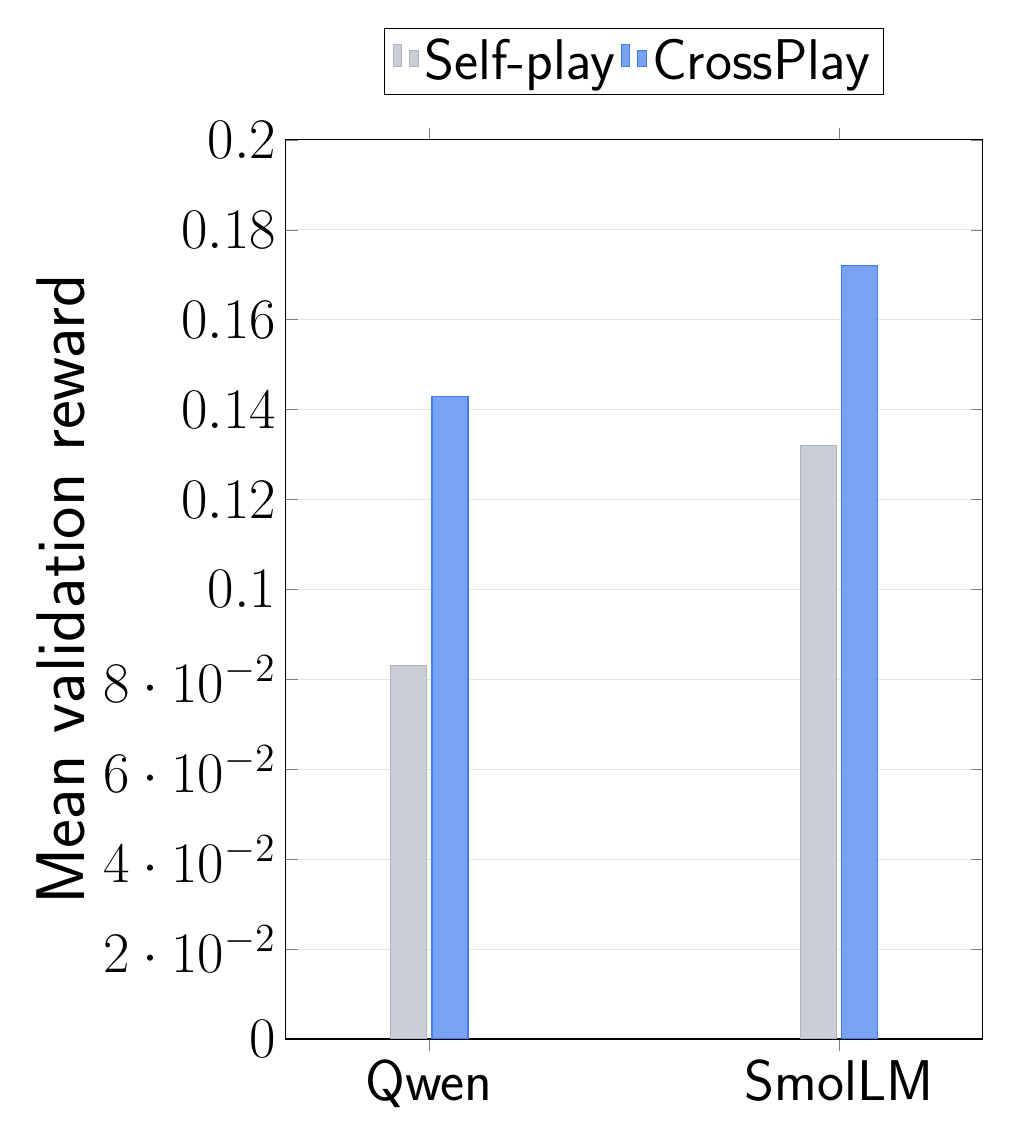
\begin{tikzpicture}
\begin{axis}[
  width=\ResultPlotWidth,
  height=\ResultPlotHeight,
  ybar,
  bar width=13pt,
  ymin=0,
  ymax=0.20,
  symbolic x coords={Qwen,SmolLM},
  xtick=data,
  ylabel={Mean validation reward},
  ylabel style={font=\fontsize{23}{27}\selectfont},
  tick label style={font=\fontsize{21}{25}\selectfont},
  legend style={font=\fontsize{20}{24}\selectfont,at={(0.5,1.05)},anchor=south,legend columns=2},
  enlarge x limits=0.35,
  ymajorgrids=true,
  grid style={linegray!35}
]
\addplot+[fill=linegray!65,draw=linegray] coordinates {(Qwen,\selfQwenReward) (SmolLM,\selfSmolReward)};
\addplot+[fill=dmblue!70,draw=dmblue] coordinates {(Qwen,\crossAReward) (SmolLM,\crossBReward)};
\legend{Self-play,CrossPlay}
\end{axis}
\end{tikzpicture}
\end{center}
\ResultTable{
\begin{tabular}{@{}llccc@{}}
\toprule
Model & Metric & Self$^\dagger$ & CP & $\Delta$ \\
\midrule
Qwen & win & \selfQwenWin & \crossAWin & $+0.055$ \\
Qwen & reward & \selfQwenReward & \crossAReward & $+0.0599$ \\
SmolLM & win & \selfSmolWin & \crossBWin & $+0.051$ \\
SmolLM & reward & \selfSmolReward & \crossBReward & $+0.0401$ \\
\bottomrule
\end{tabular}
}
\end{minipage}
\hfill
\begin{minipage}[t]{0.318\linewidth}
\MiniTitle{Balance Audit}
\ResultTable{
\begin{tabular}{@{}lcc@{}}
\toprule
Quantity & $A-B$ & Removed \\
\midrule
Replay & 0 & data volume \\
DPO pairs & 0 & pair count \\
Updates & 0 & optimizer exposure \\
\bottomrule
\end{tabular}
}
{\fontsize{20.5}{25}\selectfont
\Key{Interpretation.} The main accounting confound is removed: neither policy receives more replay data, DPO pairs, or optimizer steps. Under this audit, the measured contrast is same-family self-play versus heterogeneous online CrossPlay.}

\vspace{0.30em}

{\fontsize{20.5}{25}\selectfont
\Key{Evaluation protocol.} Validation reports win/tie rates and dense verifier rewards on the same held-out GSM8K prompts; self-play numbers are marked as provisional estimates.}
\end{minipage}

\vfill
{\color{linegray}\rule{\linewidth}{1.1pt}}
\vspace{0.35em}

{\fontsize{16}{19}\selectfont\color{textgray}
References: Munos, Valko, Calandriello et al., \textit{Nash Learning from Human Feedback}, ICML 2024; Calandriello, Guo, Munos et al., \textit{Human Alignment of LLMs through Online Preference Optimisation}, ICML 2024; Wu, Sun, Yuan, Ji, Yang, Gu, \textit{Self-Play Preference Optimization for Language Model Alignment}, 2024; Rafailov, Sharma, Mitchell, Manning, Ermon, Finn, \textit{Direct Preference Optimization}, NeurIPS 2023. $^\dagger$Self-play values are provisional estimates.
}

\end{document}
